
                \begin{figure}
                    \centering
                    \begin{tikzpicture}
                        \pgfplotsset{%
                            width=1\textwidth,
                            height=0.4\textheight
                        }
                        \begin{axis}[
                            xlabel={Start temperature},
                            ylabel={Average dynamic energy (watt)},
                            ymin=0,ymax=100,
                        ]
                        
                            \addplot [mark=none, densely dashed, red]  coordinates {
                            (35, 0.1666519654415769)(40, 0.07486629563767547)(45, 0.07859919132391237)(50, 0.07235462756748967)
                            };
                            \addlegendentry{WRK - IPG}
                            
                            \addplot [mark=none, densely dashed, blue]  coordinates {
                            (40, 0.10983094020747419)(45, 0.07954361912827101)(50, 0.07340306661669146)(55, 0.09084863970902257)
                            };
                            \addlegendentry{WRK - LHM}
                            
                            \addplot [mark=none, densely dashed, cyan]  coordinates {
                            (40, 0.0)(45, 0.0)(50, 0.0)(55, 0.0)
                            };
                            \addlegendentry{WRK - CLAMP (win)}
                            
                        \end{axis}
                    \end{tikzpicture} 
                \caption{A graph illustrating the energy consumption of Dram for test case BinaryTrees with regards to the temperature of the DUT, experiment \#2, (with outliers)} \label{fig:BinaryTrees_Dram_temperature_exp2}
                \end{figure}
                